\documentclass[]{book}
\usepackage{lmodern}
\usepackage{amssymb,amsmath}
\usepackage{ifxetex,ifluatex}
\usepackage{fixltx2e} % provides \textsubscript
\ifnum 0\ifxetex 1\fi\ifluatex 1\fi=0 % if pdftex
  \usepackage[T1]{fontenc}
  \usepackage[utf8]{inputenc}
\else % if luatex or xelatex
  \ifxetex
    \usepackage{mathspec}
  \else
    \usepackage{fontspec}
  \fi
  \defaultfontfeatures{Ligatures=TeX,Scale=MatchLowercase}
\fi
% use upquote if available, for straight quotes in verbatim environments
\IfFileExists{upquote.sty}{\usepackage{upquote}}{}
% use microtype if available
\IfFileExists{microtype.sty}{%
\usepackage{microtype}
\UseMicrotypeSet[protrusion]{basicmath} % disable protrusion for tt fonts
}{}
\usepackage[margin=1in]{geometry}
\usepackage{hyperref}
\hypersetup{unicode=true,
            pdftitle={Methods Comparison},
            pdfborder={0 0 0},
            breaklinks=true}
\urlstyle{same}  % don't use monospace font for urls
\usepackage{natbib}
\bibliographystyle{apalike}
\usepackage{color}
\usepackage{fancyvrb}
\newcommand{\VerbBar}{|}
\newcommand{\VERB}{\Verb[commandchars=\\\{\}]}
\DefineVerbatimEnvironment{Highlighting}{Verbatim}{commandchars=\\\{\}}
% Add ',fontsize=\small' for more characters per line
\usepackage{framed}
\definecolor{shadecolor}{RGB}{248,248,248}
\newenvironment{Shaded}{\begin{snugshade}}{\end{snugshade}}
\newcommand{\KeywordTok}[1]{\textcolor[rgb]{0.13,0.29,0.53}{\textbf{#1}}}
\newcommand{\DataTypeTok}[1]{\textcolor[rgb]{0.13,0.29,0.53}{#1}}
\newcommand{\DecValTok}[1]{\textcolor[rgb]{0.00,0.00,0.81}{#1}}
\newcommand{\BaseNTok}[1]{\textcolor[rgb]{0.00,0.00,0.81}{#1}}
\newcommand{\FloatTok}[1]{\textcolor[rgb]{0.00,0.00,0.81}{#1}}
\newcommand{\ConstantTok}[1]{\textcolor[rgb]{0.00,0.00,0.00}{#1}}
\newcommand{\CharTok}[1]{\textcolor[rgb]{0.31,0.60,0.02}{#1}}
\newcommand{\SpecialCharTok}[1]{\textcolor[rgb]{0.00,0.00,0.00}{#1}}
\newcommand{\StringTok}[1]{\textcolor[rgb]{0.31,0.60,0.02}{#1}}
\newcommand{\VerbatimStringTok}[1]{\textcolor[rgb]{0.31,0.60,0.02}{#1}}
\newcommand{\SpecialStringTok}[1]{\textcolor[rgb]{0.31,0.60,0.02}{#1}}
\newcommand{\ImportTok}[1]{#1}
\newcommand{\CommentTok}[1]{\textcolor[rgb]{0.56,0.35,0.01}{\textit{#1}}}
\newcommand{\DocumentationTok}[1]{\textcolor[rgb]{0.56,0.35,0.01}{\textbf{\textit{#1}}}}
\newcommand{\AnnotationTok}[1]{\textcolor[rgb]{0.56,0.35,0.01}{\textbf{\textit{#1}}}}
\newcommand{\CommentVarTok}[1]{\textcolor[rgb]{0.56,0.35,0.01}{\textbf{\textit{#1}}}}
\newcommand{\OtherTok}[1]{\textcolor[rgb]{0.56,0.35,0.01}{#1}}
\newcommand{\FunctionTok}[1]{\textcolor[rgb]{0.00,0.00,0.00}{#1}}
\newcommand{\VariableTok}[1]{\textcolor[rgb]{0.00,0.00,0.00}{#1}}
\newcommand{\ControlFlowTok}[1]{\textcolor[rgb]{0.13,0.29,0.53}{\textbf{#1}}}
\newcommand{\OperatorTok}[1]{\textcolor[rgb]{0.81,0.36,0.00}{\textbf{#1}}}
\newcommand{\BuiltInTok}[1]{#1}
\newcommand{\ExtensionTok}[1]{#1}
\newcommand{\PreprocessorTok}[1]{\textcolor[rgb]{0.56,0.35,0.01}{\textit{#1}}}
\newcommand{\AttributeTok}[1]{\textcolor[rgb]{0.77,0.63,0.00}{#1}}
\newcommand{\RegionMarkerTok}[1]{#1}
\newcommand{\InformationTok}[1]{\textcolor[rgb]{0.56,0.35,0.01}{\textbf{\textit{#1}}}}
\newcommand{\WarningTok}[1]{\textcolor[rgb]{0.56,0.35,0.01}{\textbf{\textit{#1}}}}
\newcommand{\AlertTok}[1]{\textcolor[rgb]{0.94,0.16,0.16}{#1}}
\newcommand{\ErrorTok}[1]{\textcolor[rgb]{0.64,0.00,0.00}{\textbf{#1}}}
\newcommand{\NormalTok}[1]{#1}
\usepackage{longtable,booktabs}
\usepackage{graphicx,grffile}
\makeatletter
\def\maxwidth{\ifdim\Gin@nat@width>\linewidth\linewidth\else\Gin@nat@width\fi}
\def\maxheight{\ifdim\Gin@nat@height>\textheight\textheight\else\Gin@nat@height\fi}
\makeatother
% Scale images if necessary, so that they will not overflow the page
% margins by default, and it is still possible to overwrite the defaults
% using explicit options in \includegraphics[width, height, ...]{}
\setkeys{Gin}{width=\maxwidth,height=\maxheight,keepaspectratio}
\IfFileExists{parskip.sty}{%
\usepackage{parskip}
}{% else
\setlength{\parindent}{0pt}
\setlength{\parskip}{6pt plus 2pt minus 1pt}
}
\setlength{\emergencystretch}{3em}  % prevent overfull lines
\providecommand{\tightlist}{%
  \setlength{\itemsep}{0pt}\setlength{\parskip}{0pt}}
\setcounter{secnumdepth}{5}
% Redefines (sub)paragraphs to behave more like sections
\ifx\paragraph\undefined\else
\let\oldparagraph\paragraph
\renewcommand{\paragraph}[1]{\oldparagraph{#1}\mbox{}}
\fi
\ifx\subparagraph\undefined\else
\let\oldsubparagraph\subparagraph
\renewcommand{\subparagraph}[1]{\oldsubparagraph{#1}\mbox{}}
\fi

%%% Use protect on footnotes to avoid problems with footnotes in titles
\let\rmarkdownfootnote\footnote%
\def\footnote{\protect\rmarkdownfootnote}

%%% Change title format to be more compact
\usepackage{titling}

% Create subtitle command for use in maketitle
\newcommand{\subtitle}[1]{
  \posttitle{
    \begin{center}\large#1\end{center}
    }
}

\setlength{\droptitle}{-2em}

  \title{Methods Comparison}
    \pretitle{\vspace{\droptitle}\centering\huge}
  \posttitle{\par}
    \author{Malu Calle Rosingana\\
Coding: Yiwen Wang}
    \preauthor{\centering\large\emph}
  \postauthor{\par}
      \predate{\centering\large\emph}
  \postdate{\par}
    \date{2019-05-14}

\usepackage{booktabs}
\usepackage{amsthm}
\makeatletter
\def\thm@space@setup{%
  \thm@preskip=8pt plus 2pt minus 4pt
  \thm@postskip=\thm@preskip
}
\makeatother


\usepackage{fancyhdr}
\usepackage{hyperref}
\usepackage{lipsum}
\setlength{\headheight}{28pt}
\setlength{\footskip}{25pt}
\pagestyle{fancy}
\renewcommand{\headrulewidth}{0.5pt}
\renewcommand{\footrulewidth}{0.5pt}
\lhead{
\includegraphics[width=10cm,height=1.2cm]{logo.pdf}}
\cfoot{\scriptsize Universitat de Vic | Univerisitat Central de Catalunya}
\rfoot{\scriptsize \thepage}
\fancyhead[R]{\slshape\leftmark}
\fancypagestyle{plain}{\pagestyle{fancy}}

\usepackage{fontspec}
\setmainfont{Times New Roman}

\begin{document}
\maketitle

{
\setcounter{tocdepth}{3}
\tableofcontents
}
\chapter{Introduction}\label{introduction}

This vignette provides a comparison of the 12 variables selected by the
3 methods:

\begin{itemize}
\tightlist
\item
  logistic\_lasso + linear constraints;
\item
  centered logratio transformation (CLR) + logistic\_lasso;
\item
  selbal.
\end{itemize}

First, you will need to install then load the following packages:

\section{Packages installation and
loading}\label{packages-installation-and-loading}

\begin{Shaded}
\begin{Highlighting}[]
\CommentTok{#cran.packages <- c('knitr', 'MASS', 'VennDiagram', 'gplots', 'glmnet')}
\CommentTok{#install.packages(cran.packages)}
\CommentTok{#devtools::install_github(repo = "UVic-omics/selbal")}

\KeywordTok{library}\NormalTok{(knitr) }\CommentTok{# rbookdown}
\KeywordTok{library}\NormalTok{(MASS) }\CommentTok{# ginv}
\KeywordTok{library}\NormalTok{(VennDiagram) }\CommentTok{# venn.diagram}
\KeywordTok{library}\NormalTok{(gplots) }\CommentTok{# venn}
\KeywordTok{library}\NormalTok{(glmnet) }\CommentTok{# glmnet}
\KeywordTok{library}\NormalTok{(selbal) }\CommentTok{# selbal}

\CommentTok{# build in functions}
\KeywordTok{source}\NormalTok{(}\DataTypeTok{file =} \StringTok{'functions.R'}\NormalTok{)}
\end{Highlighting}
\end{Shaded}

\section{Simulations}\label{simulations}

The way we simulate datasets.

\section{Example datasets}\label{example-datasets}

We have two case studies.

\subsection{Microbiome and Crohn's
disease}\label{microbiome-and-crohns-disease}

Crohn's disease (CD) is an inflammatory bowel disease that has been
linked to microbial alterations in the gut
\citep{gevers2014treatment, oyri2015dysbiotic}. We use data from a large
pediatric CD cohort study \citep{gevers2014treatment} to compare the
proposed methodologies for identification of microbial signatures.

Microbiome data from 16S rRNA gene sequencing and QIIME 1.7.0
bioinformatics processing were downloaded from Qiita
\citep{rivera2018balances}. Only patients with Crohn's disease (n = 662)
and those without any symptoms (n = 313) were analyzed. The OTU table
was agglomerated to the genus level, resulting in a matrix with 48
genera and 975 samples.

We load the data that are provided in advance.

\begin{Shaded}
\begin{Highlighting}[]
\KeywordTok{load}\NormalTok{(}\StringTok{"./datasets/Crohn_data.rda"}\NormalTok{)}
\CommentTok{# dim(x_Crohn)}
\CommentTok{# summary(y_Crohn)}
\end{Highlighting}
\end{Shaded}

\begin{longtable}[]{@{}cc@{}}
\caption{\textbf{CD data summary}}\tabularnewline
\toprule
No. of genera & 48\tabularnewline
No. of samples & 975\tabularnewline
No. of patients with CD & 662\tabularnewline
No. of healthy patients & 313\tabularnewline
\bottomrule
\end{longtable}

\subsection{BEME day1 data}\label{beme-day1-data}

content need to be added.

\chapter{CODA\_LOGISTIC\_LASSO}\label{coda}

First, we illustrate the method lasso with linear constraints.

\section{CD data}\label{cd-data}

\begin{Shaded}
\begin{Highlighting}[]
\NormalTok{x <-}\StringTok{ }\NormalTok{x_Crohn }
\end{Highlighting}
\end{Shaded}

x is the matrix of microbiome abundances, either absolute abundances
(counts) or relative abundances (proportions). However, x should not be
the matrix of log(counts) or log(proportions). The method itself
performs the log-transformation of the abundances.

\begin{Shaded}
\begin{Highlighting}[]
\NormalTok{y <-}\StringTok{ }\NormalTok{y_Crohn }
\KeywordTok{summary}\NormalTok{(y)}
\end{Highlighting}
\end{Shaded}

\begin{verbatim}
##  CD  no 
## 662 313
\end{verbatim}

In the CD data, y is the binary outcome, can be numerical (values 0 and
1), factor (2 levels) or categorical (2 categories).

\begin{Shaded}
\begin{Highlighting}[]
\KeywordTok{dim}\NormalTok{(x)}
\end{Highlighting}
\end{Shaded}

\begin{verbatim}
## [1] 975  48
\end{verbatim}

The rows of x are individuals/samples, the columns are taxa.

To run the method, we need a value of \(\lambda\).

\begin{Shaded}
\begin{Highlighting}[]
\KeywordTok{rangLambda}\NormalTok{(y, x,}\DataTypeTok{numVar =} \DecValTok{12}\NormalTok{, }\DataTypeTok{lambdaIni =} \FloatTok{0.15}\NormalTok{)}
\end{Highlighting}
\end{Shaded}

\begin{verbatim}
## [1]  0.00  0.65 48.00 17.00
## [1]  0.000  0.325 48.000  2.000
## [1]  0.1625  0.3250 12.0000  2.0000
\end{verbatim}

\begin{verbatim}
## $`rang lambdas`
## [1] 0.1625 0.3250
## 
## $`num selected variables`
## [1] 12  2
\end{verbatim}

It provides a rang of \(\lambda\) values corresponding to a given number
of variables to be selected (numVar).

The default initial \(\lambda\) is lambdaIni=1.

\begin{Shaded}
\begin{Highlighting}[]
\NormalTok{results_codalasso <-}\StringTok{ }\KeywordTok{coda_logistic_lasso}\NormalTok{(y, x, }\DataTypeTok{lambda =} \FloatTok{0.19}\NormalTok{)}
\end{Highlighting}
\end{Shaded}

\(\lambda\) is the penalization parameter: the larger the value of
\(\lambda\), the fewer number of variables will be selected.

\begin{Shaded}
\begin{Highlighting}[]
\NormalTok{results_codalasso}
\end{Highlighting}
\end{Shaded}

\begin{verbatim}
## $`number of iterations`
## [1] 23
## 
## $`number of selected taxa`
## [1] 11
## 
## $`indices of taxa with non-zero coeff`
##  [1]  0  2  5  9 19 27 31 32 33 39 40 48
## 
## $`taxa with non-zero coeff`
##  [1] "beta0"                        "g__Parabacteroides"          
##  [3] "f__Peptostreptococcaceae_g__" "g__Eggerthella"              
##  [5] "g__Dialister"                 "o__Lactobacillales_g__"      
##  [7] "g__Prevotella"                "g__Roseburia"                
##  [9] "g__Lachnospira"               "g__Streptococcus"            
## [11] "g__Aggregatibacter"           "g__Bilophila"                
## 
## $`beta non-zero coefficients`
##  [1] -1.0023255478 -0.0057464016  0.0202907034 -0.0184875313 -0.0992393846
##  [6] -0.0159418386 -0.0030842274  0.2530005235 -0.0085670215 -0.0818265310
## [11] -0.0406982632  0.0002999724
## 
## $`proportion of explained deviance`
## [1] 0.1542276
## 
## $betas
##  [1] -1.0023255478  0.0000000000 -0.0057464016  0.0000000000  0.0000000000
##  [6]  0.0202907034  0.0000000000  0.0000000000  0.0000000000 -0.0184875313
## [11]  0.0000000000  0.0000000000  0.0000000000  0.0000000000  0.0000000000
## [16]  0.0000000000  0.0000000000  0.0000000000  0.0000000000 -0.0992393846
## [21]  0.0000000000  0.0000000000  0.0000000000  0.0000000000  0.0000000000
## [26]  0.0000000000  0.0000000000 -0.0159418386  0.0000000000  0.0000000000
## [31]  0.0000000000 -0.0030842274  0.2530005235 -0.0085670215  0.0000000000
## [36]  0.0000000000  0.0000000000  0.0000000000  0.0000000000 -0.0818265310
## [41] -0.0406982632  0.0000000000  0.0000000000  0.0000000000  0.0000000000
## [46]  0.0000000000  0.0000000000  0.0000000000  0.0002999724
\end{verbatim}

\begin{Shaded}
\begin{Highlighting}[]
\NormalTok{selected_codalasso <-}\StringTok{ }\NormalTok{results_codalasso[[}\DecValTok{4}\NormalTok{]][}\OperatorTok{-}\DecValTok{1}\NormalTok{]}

\NormalTok{columns_selected_codalasso <-}\StringTok{ }\NormalTok{results_codalasso[[}\DecValTok{3}\NormalTok{]][}\OperatorTok{-}\DecValTok{1}\NormalTok{]}

\KeywordTok{write.csv}\NormalTok{(}\KeywordTok{data.frame}\NormalTok{(columns_selected_codalasso,selected_codalasso),}
          \StringTok{"./Generated_datasets/results_codalasso_Crohn12.csv"}\NormalTok{)}
\end{Highlighting}
\end{Shaded}

We extract the name of selected genera and their column indices and then
save them in a csv file.

\section{BEME day1 data}\label{beme-day1-data-1}

content need to be added.

\chapter{CLR\_LOGISTIC\_LASSO}\label{clr}

Then, we illustrate a combined method with centered logratio
transformation (CLR) and lasso.

\section{CD data}\label{cd-data-1}

\begin{Shaded}
\begin{Highlighting}[]
\NormalTok{x <-}\StringTok{ }\KeywordTok{as.matrix}\NormalTok{(x_Crohn)}
\NormalTok{y <-}\StringTok{ }\NormalTok{y_Crohn_numeric }
\end{Highlighting}
\end{Shaded}

Here, y is numeric, because \emph{glmnet()} requires y to be numeric.

\begin{Shaded}
\begin{Highlighting}[]
\CommentTok{# CLR transformation Z=log(x)}
\NormalTok{z <-}\StringTok{ }\KeywordTok{log}\NormalTok{(x)}
\NormalTok{clrx <-}\StringTok{ }\KeywordTok{apply}\NormalTok{(z, }\DecValTok{2}\NormalTok{, }\ControlFlowTok{function}\NormalTok{(x) x}\OperatorTok{-}\KeywordTok{rowMeans}\NormalTok{(z))}
\CommentTok{# rowMeans(clrx)  }
\end{Highlighting}
\end{Shaded}

x (the matrix of microbiome abundances) is then CLR transformed.

\begin{Shaded}
\begin{Highlighting}[]
\NormalTok{clrlasso <-}\StringTok{ }\KeywordTok{glmnet}\NormalTok{(clrx, y, }\DataTypeTok{standardize =} \OtherTok{FALSE}\NormalTok{, }\DataTypeTok{alpha =} \DecValTok{1}\NormalTok{,}\DataTypeTok{family =} \StringTok{"binomial"}\NormalTok{, }
                   \DataTypeTok{lambda =} \KeywordTok{seq}\NormalTok{(}\FloatTok{0.015}\NormalTok{, }\DecValTok{2}\NormalTok{, }\FloatTok{0.01}\NormalTok{)) }
\KeywordTok{plot}\NormalTok{(clrlasso)}
\end{Highlighting}
\end{Shaded}

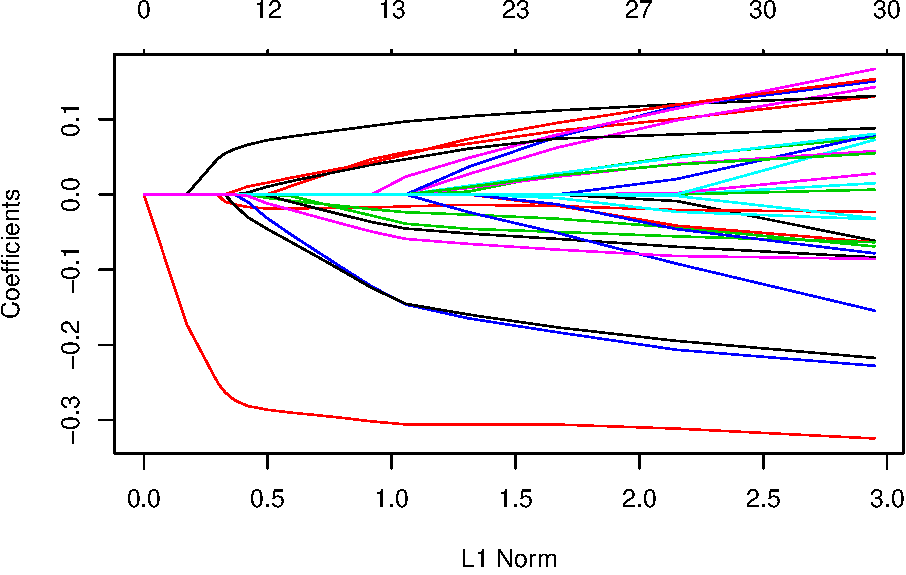
\includegraphics{Methods_comparison_files/figure-latex/unnamed-chunk-11-1.pdf}

\begin{Shaded}
\begin{Highlighting}[]
\CommentTok{#print(clrlasso)}
\NormalTok{clrlasso_coef <-}\StringTok{ }\KeywordTok{coef}\NormalTok{(clrlasso, }\DataTypeTok{s =} \FloatTok{0.10}\NormalTok{)}
\KeywordTok{sum}\NormalTok{(}\KeywordTok{abs}\NormalTok{(clrlasso_coef) }\OperatorTok{>}\StringTok{ }\DecValTok{0}\NormalTok{)}
\end{Highlighting}
\end{Shaded}

\begin{verbatim}
## [1] 13
\end{verbatim}

\begin{Shaded}
\begin{Highlighting}[]
\NormalTok{selected_clrlasso <-}\StringTok{ }\KeywordTok{which}\NormalTok{(}\KeywordTok{as.numeric}\NormalTok{(}\KeywordTok{abs}\NormalTok{(}\KeywordTok{coef}\NormalTok{(clrlasso, }\DataTypeTok{s =} \FloatTok{0.1}\NormalTok{))) }\OperatorTok{>}\StringTok{ }\DecValTok{0}\NormalTok{)[}\OperatorTok{-}\DecValTok{1}\NormalTok{]; }
\end{Highlighting}
\end{Shaded}

We obtain the indices of selected variables (abs(coef) \textgreater{} 0)
from lasso.

\begin{Shaded}
\begin{Highlighting}[]
\NormalTok{selected_clrlasso <-}\StringTok{ }\NormalTok{selected_clrlasso }\OperatorTok{-}\StringTok{ }\DecValTok{1}
\NormalTok{taxa_id <-}\StringTok{ }\KeywordTok{colnames}\NormalTok{(x_Crohn)[selected_clrlasso]}

\KeywordTok{write.csv}\NormalTok{(}\KeywordTok{data.frame}\NormalTok{(selected_clrlasso, taxa_id),}
          \StringTok{"./Generated_datasets/results_clrlasso_Crohn12.csv"}\NormalTok{)}
\end{Highlighting}
\end{Shaded}

The name of selected genera and their indices are also saved in a csv
file.

\section{BEME day1 data}\label{beme-day1-data-2}

content need to be added.

\chapter{Selbal: selection of balances}\label{selbal}

The last method to illustrate is selbal, see details in
\citep{rivera2018balances}.

\section{CD data}\label{cd-data-2}

\begin{Shaded}
\begin{Highlighting}[]
\NormalTok{x <-}\StringTok{ }\NormalTok{x_Crohn }
\KeywordTok{colnames}\NormalTok{(x) <-}\StringTok{ }\NormalTok{(}\DecValTok{1}\OperatorTok{:}\KeywordTok{ncol}\NormalTok{(x))}

\NormalTok{y <-}\StringTok{ }\NormalTok{y_Crohn  }
\end{Highlighting}
\end{Shaded}

For binary outcomes (logistic regression), \emph{selbal()} requires y to
be factor. If y is numeric, \emph{selbal()} implements linear
regression.

\begin{Shaded}
\begin{Highlighting}[]
\NormalTok{selbal_Crohn <-}\StringTok{ }\KeywordTok{selbal}\NormalTok{(}\DataTypeTok{x =}\NormalTok{ x, }\DataTypeTok{y =}\NormalTok{ y, }\DataTypeTok{logt=}\NormalTok{T, }\DataTypeTok{maxV=}\DecValTok{12}\NormalTok{)}
\end{Highlighting}
\end{Shaded}

\begin{figure}
\centering
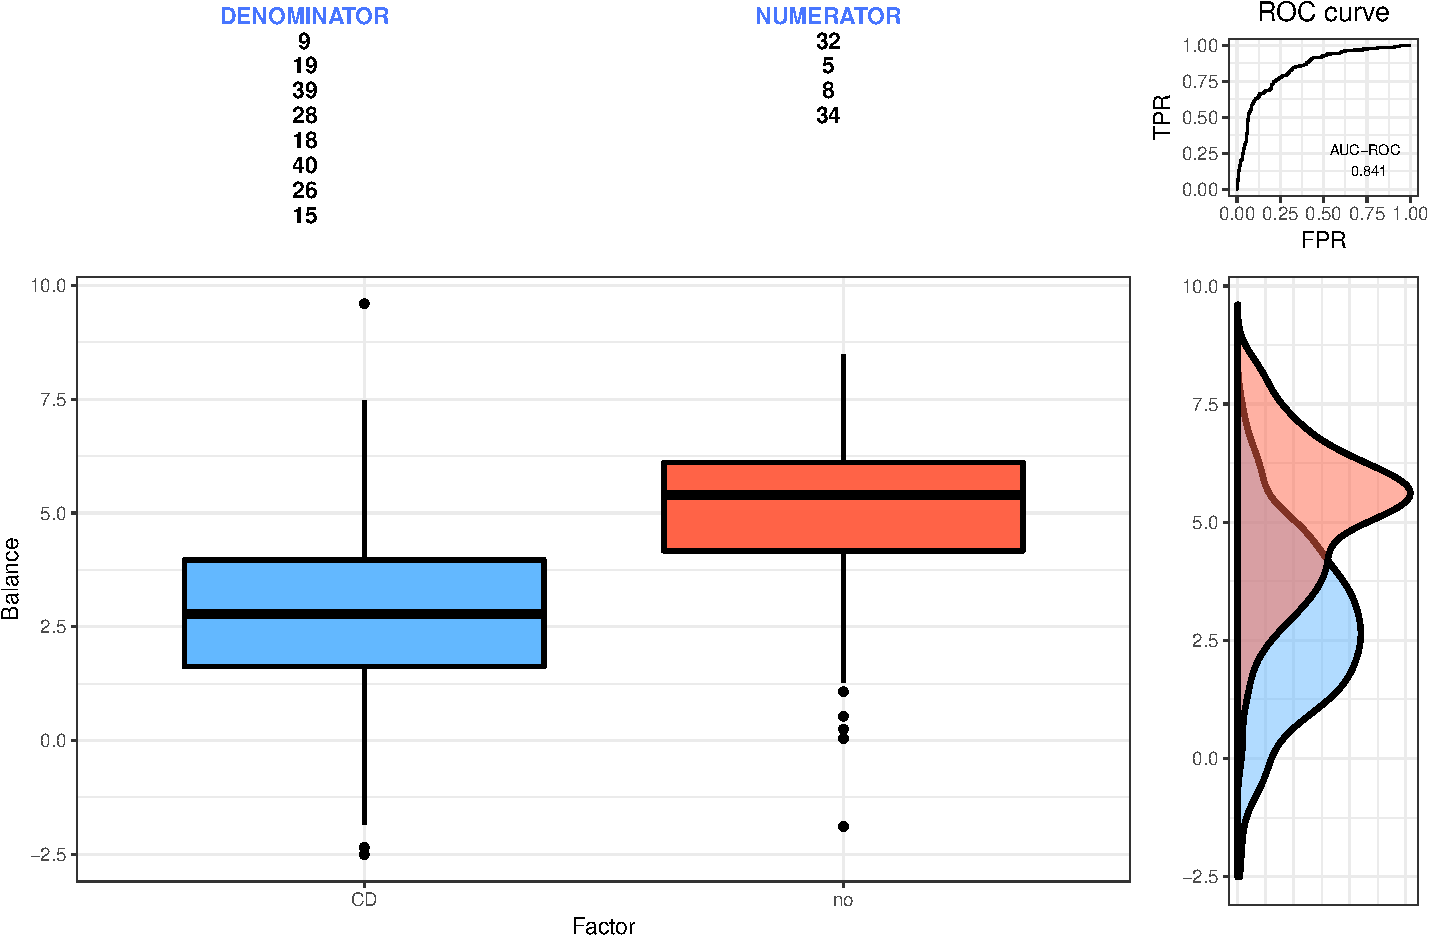
\includegraphics{Methods_comparison_files/figure-latex/selbalfig-1.pdf}
\caption{\label{fig:selbalfig}Description of the global balance for CD.}
\end{figure}

We use \textbf{A}rea \textbf{U}nder the receiver operating
characteristic \textbf{C}urve (AUC) to deciede what is the optimal
number of variables. Once the first two-taxon balance is selected, the
algorithm performs a forward selection process. At each step, a new
taxon is added to the existing balance such that AUC is improved, the
algorithm stops when there is no additional variable that increase the
current AUC or when the maximun number of variables to be included in
the balance is achieved.

In Figure \ref{fig:selbalfig}, the two groups of taxa that form the
global balance are specified at the top of the plot. The box plot
represents the distribution of the balance scores for CD and non-CD
individuals. The right part of the figure contains the ROC curve with
its AUC value and the density curve for each group.

\begin{Shaded}
\begin{Highlighting}[]
\NormalTok{selected_selbal <-}\StringTok{ }\KeywordTok{as.numeric}\NormalTok{(}\KeywordTok{c}\NormalTok{(selbal_Crohn[[}\DecValTok{6}\NormalTok{]][,}\DecValTok{1}\NormalTok{], selbal_Crohn[[}\DecValTok{6}\NormalTok{]][,}\DecValTok{2}\NormalTok{]))}
\NormalTok{id.na <-}\StringTok{ }\KeywordTok{which}\NormalTok{(}\KeywordTok{is.na}\NormalTok{(selected_selbal))}
\NormalTok{selected_selbal <-}\StringTok{ }\NormalTok{selected_selbal[}\OperatorTok{-}\NormalTok{id.na]}
\NormalTok{selected_selbal <-}\StringTok{ }\KeywordTok{as.character}\NormalTok{(selected_selbal)}

\NormalTok{columns_selected_selbal <-}\StringTok{ }\KeywordTok{which}\NormalTok{(}\KeywordTok{colnames}\NormalTok{(x)}\OperatorTok\StringTok{ }\NormalTok{selected_selbal)}
\NormalTok{taxa_id <-}\StringTok{ }\KeywordTok{colnames}\NormalTok{(x_Crohn)[columns_selected_selbal]}

\KeywordTok{write.csv}\NormalTok{(}\KeywordTok{data.frame}\NormalTok{(columns_selected_selbal, taxa_id),}
          \StringTok{"./Generated_datasets/results_selbal_Crohn12.csv"}\NormalTok{)}
\end{Highlighting}
\end{Shaded}

The name of selected genera and their indices are also saved as the
other method did.

\section{BEME day1 data}\label{beme-day1-data-3}

content need to be added.

\chapter{Concordance of variables selected by the three
methods}\label{comparison}

\section{CD data}\label{cd-data-3}

\begin{Shaded}
\begin{Highlighting}[]
\NormalTok{d_selbal <-}\StringTok{ }\KeywordTok{read.csv}\NormalTok{(}\StringTok{"./Generated_datasets/results_selbal_Crohn12.csv"}\NormalTok{, }\DataTypeTok{header =}\NormalTok{ T)}
\NormalTok{d_clrlasso <-}\StringTok{ }\KeywordTok{read.csv}\NormalTok{(}\StringTok{"./Generated_datasets/results_clrlasso_Crohn12.csv"}\NormalTok{, }\DataTypeTok{header =}\NormalTok{ T)}
\NormalTok{d_codalasso <-}\StringTok{ }\KeywordTok{read.csv}\NormalTok{(}\StringTok{"./Generated_datasets/results_codalasso_Crohn12.csv"}\NormalTok{, }\DataTypeTok{header =}\NormalTok{ T)}
  
\NormalTok{taxa_selected <-}\StringTok{ }\KeywordTok{list}\NormalTok{(d_clrlasso[,}\DecValTok{2}\NormalTok{], d_codalasso[,}\DecValTok{2}\NormalTok{], d_selbal[,}\DecValTok{2}\NormalTok{])}
\NormalTok{taxa.id_selected <-}\StringTok{ }\KeywordTok{list}\NormalTok{(d_clrlasso[,}\DecValTok{3}\NormalTok{], d_codalasso[,}\DecValTok{3}\NormalTok{], d_selbal[,}\DecValTok{3}\NormalTok{])}


\NormalTok{venn.plot <-}\StringTok{ }\KeywordTok{venn.diagram}\NormalTok{(taxa_selected, }\OtherTok{NULL}\NormalTok{, }\DataTypeTok{fill =} \KeywordTok{c}\NormalTok{(}\StringTok{"magenta"}\NormalTok{, }\StringTok{"blue"}\NormalTok{, }\StringTok{"lightblue"}\NormalTok{), }
                          \DataTypeTok{alpha=}\KeywordTok{c}\NormalTok{(}\FloatTok{0.5}\NormalTok{,}\FloatTok{0.5}\NormalTok{,}\FloatTok{0.5}\NormalTok{), }\DataTypeTok{cex =} \DecValTok{2}\NormalTok{, }\DataTypeTok{cat.fontface=}\DecValTok{4}\NormalTok{, }
                          \DataTypeTok{category.names =} \KeywordTok{c}\NormalTok{(}\StringTok{"clr+lasso"}\NormalTok{, }\StringTok{"coda-lasso"}\NormalTok{, }\StringTok{"selbal"}\NormalTok{),}
                          \DataTypeTok{main =} \StringTok{"Concordance of selected taxa for Crohn data"}\NormalTok{)}
\KeywordTok{grid.draw}\NormalTok{(venn.plot)}
\end{Highlighting}
\end{Shaded}

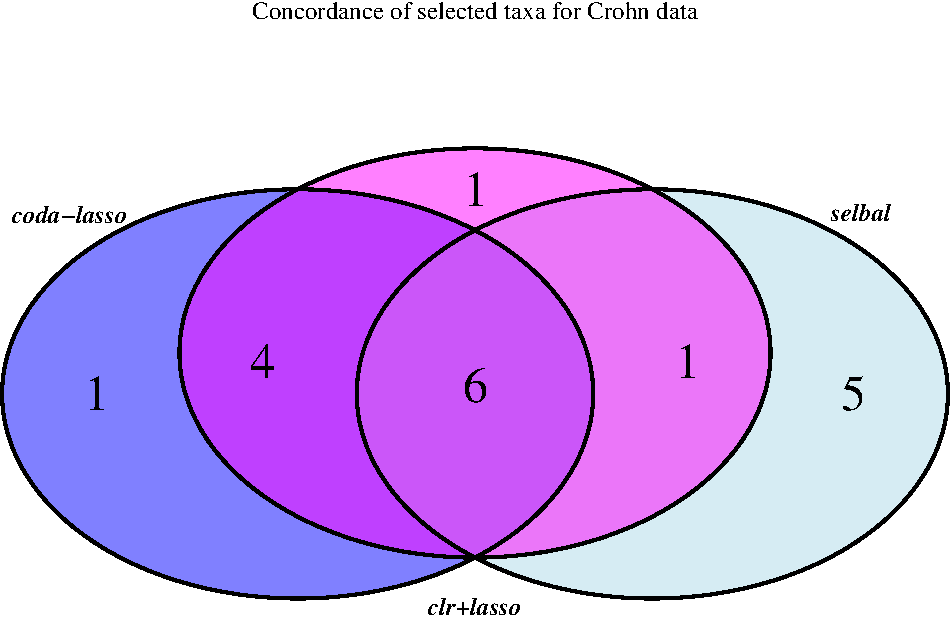
\includegraphics{Methods_comparison_files/figure-latex/unnamed-chunk-15-1.pdf}

\begin{Shaded}
\begin{Highlighting}[]
\NormalTok{taxa.id <-}\StringTok{ }\KeywordTok{venn}\NormalTok{(taxa.id_selected, }\DataTypeTok{show.plot=}\OtherTok{FALSE}\NormalTok{)}
\NormalTok{taxa <-}\StringTok{ }\KeywordTok{venn}\NormalTok{(taxa_selected, }\DataTypeTok{show.plot=}\OtherTok{FALSE}\NormalTok{)}

\NormalTok{inters_taxa.id <-}\StringTok{ }\KeywordTok{attr}\NormalTok{(taxa.id, }\StringTok{"intersections"}\NormalTok{)}
\NormalTok{inters_taxa <-}\StringTok{ }\KeywordTok{attr}\NormalTok{(taxa, }\StringTok{"intersections"}\NormalTok{)}

\KeywordTok{lapply}\NormalTok{(inters_taxa, head) }
\end{Highlighting}
\end{Shaded}

\begin{verbatim}
## $A
## [1] "10"
## 
## $B
## [1] "27"
## 
## $C
## [1] "15" "18" "26" "28" "34"
## 
## $`A:B`
## [1] "2"  "31" "33" "48"
## 
## $`A:C`
## [1] "8"
## 
## $`A:B:C`
## [1] "5"  "9"  "19" "32" "39" "40"
\end{verbatim}

\begin{Shaded}
\begin{Highlighting}[]
\KeywordTok{lapply}\NormalTok{(inters_taxa.id, head) }
\end{Highlighting}
\end{Shaded}

\begin{verbatim}
## $A
## [1] "g__Faecalibacterium"
## 
## $B
## [1] "o__Lactobacillales_g__"
## 
## $C
## [1] "g__Blautia"           "g__Dorea"             "g__Oscillospira"     
## [4] "g__Adlercreutzia"     "o__Clostridiales_g__"
## 
## $`A:B`
## [1] "g__Parabacteroides" "g__Prevotella"      "g__Lachnospira"    
## [4] "g__Bilophila"      
## 
## $`A:C`
## [1] "g__Bacteroides"
## 
## $`A:B:C`
## [1] "f__Peptostreptococcaceae_g__" "g__Eggerthella"              
## [3] "g__Dialister"                 "g__Roseburia"                
## [5] "g__Streptococcus"             "g__Aggregatibacter"
\end{verbatim}

need more explanation of the venn diagram.

\section{BEME day1 data}\label{beme-day1-data-4}

content need to be added.

\bibliography{book.bib}


\end{document}
